\documentclass{article}

\usepackage{graphicx}
\usepackage{geometry}
\geometry{
  a4paper,
  total={170mm,257mm},
  left=20mm,
  top=20mm,
}
\usepackage{crimson}
\usepackage[T1]{fontenc}
\usepackage[round]{natbib}
\usepackage{nameref}

\title{Evaluating contact tracing and isolation to control pandemic potential influenza outbreaks}
\author{Joshua W. Lambert}
\date{}

\begin{document}

\maketitle

\section*{Abstract}

\section*{Introduction}

The likelihood of an outbreak being controlled, in other words going locally-extinct or -eliminated, is in part based on the epidemiological characteristics of the pathogen, and in part on the inventions implemented, both pharmaceutical and non-pharmaceutical. The primary epidemiological determinant for the spread of an infectious disease is the reproduction number, defined as the average number of secondary cases  per primary case. The higher the reproduction number the less likely a disease, without intervention, is to cease transmission in a population. If a pathogen is subcritical (i.e. $R < 1$) it will eventually stop spreading but can still cause transient outbreaks \citep{farringtonDistributionTimeExtinction1999}. Individual-level heterogeneity in transmission also influences the possibility of a pathogen going extinct from stochasticity in the transmission process \citep{lloyd-smithSuperspreadingEffectIndividual2005}. Higher individual-level variation for a given reproduction leading to, on average, more outbreaks being controlled (however a small number of outbreaks may become large due to superspreading). In addition, the likelihood of containment is reduced (assuming $R > 1$) if there are multiple introductions into a populations \citep{kucharskiEarlyDynamicsTransmission2020}. \\

There are a variety of interventions that can be enacted to try and prevent transmission of an infectious disease, including both pharmaceutical and non-pharmaceutical interventions (NPIs). Early in an outbreak NPIs are often used, as especially for outbreaks of a novel pathogen before pharmaceutical inventions are available. These interventions range in their specificity, from targeted contact tracing which aims to tackle specific transmission pathways, to closure of school and gathering, to regional or national lockdowns affecting everyone (ref). \\

Contact tracing, the process of finding the contacts of infected individuals is an often used NPI to try and curtail the growth of an epidemic. It can involve forward contact tracing, whereby infected individuals are asked who they have in contact with so their contacts can be followed-up and isolated or quarantined is needed; or backward contact tracing whereby infected individuals are asked who they have been in contact with prior to being infected to identify the source of infection and potentially forward trace from the source. Contact tracing and isolation is a targeted approach, like ring vaccination, that looks to prevent the onward transmission of an infectious disease by tackling infected individuals and their contacts \citep{kucharskiEffectivenessRingVaccination2016} (ref). Isolation of traced individuals has proved widely effective in controlling different outbreaks with a variety of pathogens differing in their aetiological and epidemiological characteristics (SARS ref; other refs). However, it's important to remember that it's not a panacea for all outbreak scenarios. In epidemics or pandemics where the proportion of cases or contacts missed is high, either because surveillance is patchy or because the number of contacts exceeds the capacity of the system, the efficacy of contact tracing to contain an outbreak diminishes, or at worst, fails completely \citep{dhillonWhenContactTracing2018} (ref on limited capacity of tracing). \\

Outbreaks have been shown to be more easily controlled when a large proportion of onward transmission takes place after the onset of symptoms \citep{fraserFactorsThatMake2004}.

- Pandemic flu has similar pre-symptomatic transmission is similar to COVID-19 (ref).
- SI shorter for pandemic flu (ref). \\

It has become widely accepted that influenza viruses cannot be controlled with contact tracing and isolation become the rate at which infected individuals become infectious and show symptoms is faster than the latency in the process of contacting contacts (ref). However, with the recent human infections of avian influenza (A/H5N1), mostly among poultry and cattle farmers and the longer estimates of incubation period and serial interval (SI) from historical H5N1 data \citep{Ward2024.12.11.24318702} it may not be the case that contact tracing and isolation is unable to control influenza. Historically, avian influenza (H5N1 and H7N9) have had high severity (case fatality risk $\sim 35\%-55\%$), and therefore sustained transmission in a human population could have substantial mortality and morbidity implications \citep{tannerPandemicPotentialAvian2015}. \\

The (antigenic) novelty of a pathogen introduced into a human population is a leading risk factor for causing a pandemic (ref). Thus, influenza subtypes that have negligible levels of existing immunity in the population are probable epidemic and pandemic candidates. This is the case for H5N1 and H7N9 \citep{tannerPandemicPotentialAvian2015} and was the case when H1N1 caused an outbreak in 2009 (ref). \\

In this study we evaluate the effectiveness of controlling infectious disease outbreaks that exhibit influenza-like epidemiological characteristics using a mathematical model. This can be used to define the speed and effectiveness of isolation given an epidemic scenario to inform outbreak response complementing in combination with other quickly available measures for pandemic potential influenza strains, such as rapid testing and antivirals (ref).

\section*{Methods}

\subsection*{Branching process model with isolation}

To assess the efficaciousness of contact tracing and isolation to control an outbreak of pandemic-potential influenza we used an individual-level transmision model implemented in the R package \texttt{{ringbp}} \citep{hellewellRingbpSimulateEvaluate2025}. The epidemic simulation model uses a single-type branching process with a negative binomial offspring distribution to simulate the spread of a pathogen through a population (without depletion of susceptibility). The mean of the negative binomial offspring distribution is the basic reproduction number, and this distribution allows the model to be parameterised to capture overdispersion of transmission, in other words, some infectors are superspreaders and infect a disproportionate number of individuals \citep{lloyd-smithSuperspreadingEffectIndividual2005, kucharskiEarlyDynamicsTransmission2020}. \\

The NPI implemented in the transmission model is an isolation of symptomatic cases. The timing of isolation is drawn from the onset-to-isolation distribution (see \nameref{epiparameters} section for parameterisation). All infection times that are sampled to occur after the isolation of an infector are not infected. Therefore, the isolation of a case can reduce the number of secondary cases if isolation happens prior to any of the secondary infection times. \\

\subsection*{Defining outbreak control}

We use the same definition for outbreak control as \cite{hellewellFeasibilityControllingCOVID192020}: no new cases between 12 and 16 weeks after the start of an outbreak. The rationale for this criteria is that some outbreaks that do not take off and become large may still have a few cases for the first few weeks of an outbreak, therefore the window for control needs to be enough time after the seeding of an outbreak to be sure it is extinct. \\

There is also a maximum number of cases in simulation model, that when reached is judged to have reached a large epidemic and not controllable with 12-16 weeks. We set this limit to 500 cases.

\subsection*{Pathogen epidemiological parameters} \label{epiparameters}

In this study we evaluate the feasibility of controlling outbreaks of selected influenza subtypes that have previous caused sporadic human-to-human outbreaks with pandemic potential. We include A/H5N1, A/H1N1, and A/H7N9. These have caused outbreaks of various size and severity over the past 100 years. H5N1 has caused small outbreaks ($<$ 10 cases) of human-to-human transmission \citep{yangDetectingHumanhumanTransmission2007a, aditamaAvianInfluenzaH5N12012a}. H1N1 is now an endemic seasonal influenza with substantial population immunity, but a novel strain, H1N1pdm09, emerged in 2009 and caused a pandemic outbreak \citep{fraserPandemicPotentialStrain2009, lesslerOutbreak2009Pandemic2009} (ref on history of H1N1pdm). \\

We extracted incubation periods from the epidemiological literature that have been previously estimated for the chosen Influenza subtypes. All incubation periods were found to be well described by a Weibull distribution, \cite{nishiuraEstimationIncubationPeriod2011} report the best fitting Weibull shape and scale parameters for H1N1 to be 1.77 and 1.86, respectively (Figure \ref{fig:incub}). \cite{cowlingComparativeEpidemiologyHuman2013} report the incubation period for H5N1 and H7N9, both Weibull distributed. For H5N1 the Weibull distribution has a mean of 3.3 days and standard deviation (SD) of 1.5 days, for H7N9 the Weibull distribution has a mean of 3.1 days and SD 1.4 days \citep{cowlingComparativeEpidemiologyHuman2013} (Figure \ref{fig:incub}). \\

The reproduction number ($R$) use to simulate transmission for each influenza subtype was 1.1, 1.5 and 2.0. We chose these values and they represent either similar values to previously estimated $R$ values for influenza outbreaks \citep{fergusonStrategiesMitigatingInfluenza2006}, including H1N1 \citep{fraserPandemicPotentialStrain2009}, or they represent an inflated values of current estimates of H5N1 and H7N9 subtypes to evaluate the effectiveness of contact tracing and isolation in the event that pathogen evolution (e.g. recombination of subtypes (ref)) enhances the human-to-human transmissibility of these pathogens. Current estimates for H5N1 and H7N9 subtypes are below unity (i.e. $R < 1$) (\citealt{tannerPandemicPotentialAvian2015}; \citealt{Ward2024.12.11.24318702}, but see \citealt{yangDetectingHumanhumanTransmission2007a} for a H5N1 $R$ estimate above 1) so transmission is expected to stop without intervention (except in a extremely rare case of superspreading event). Therefore evaluating contact tracing and isolation requires simulating outbreaks that are likely to exponentially spread without control measures.

\begin{itemize}

\item H1N1-like
\item H5N1 (slightly increased reproduction number, R~1)
\item H7N9 (if parameters are available)

\end{itemize}

Figure for parameter space for flu-like pandemic


\begin{figure}[ht]
\centering
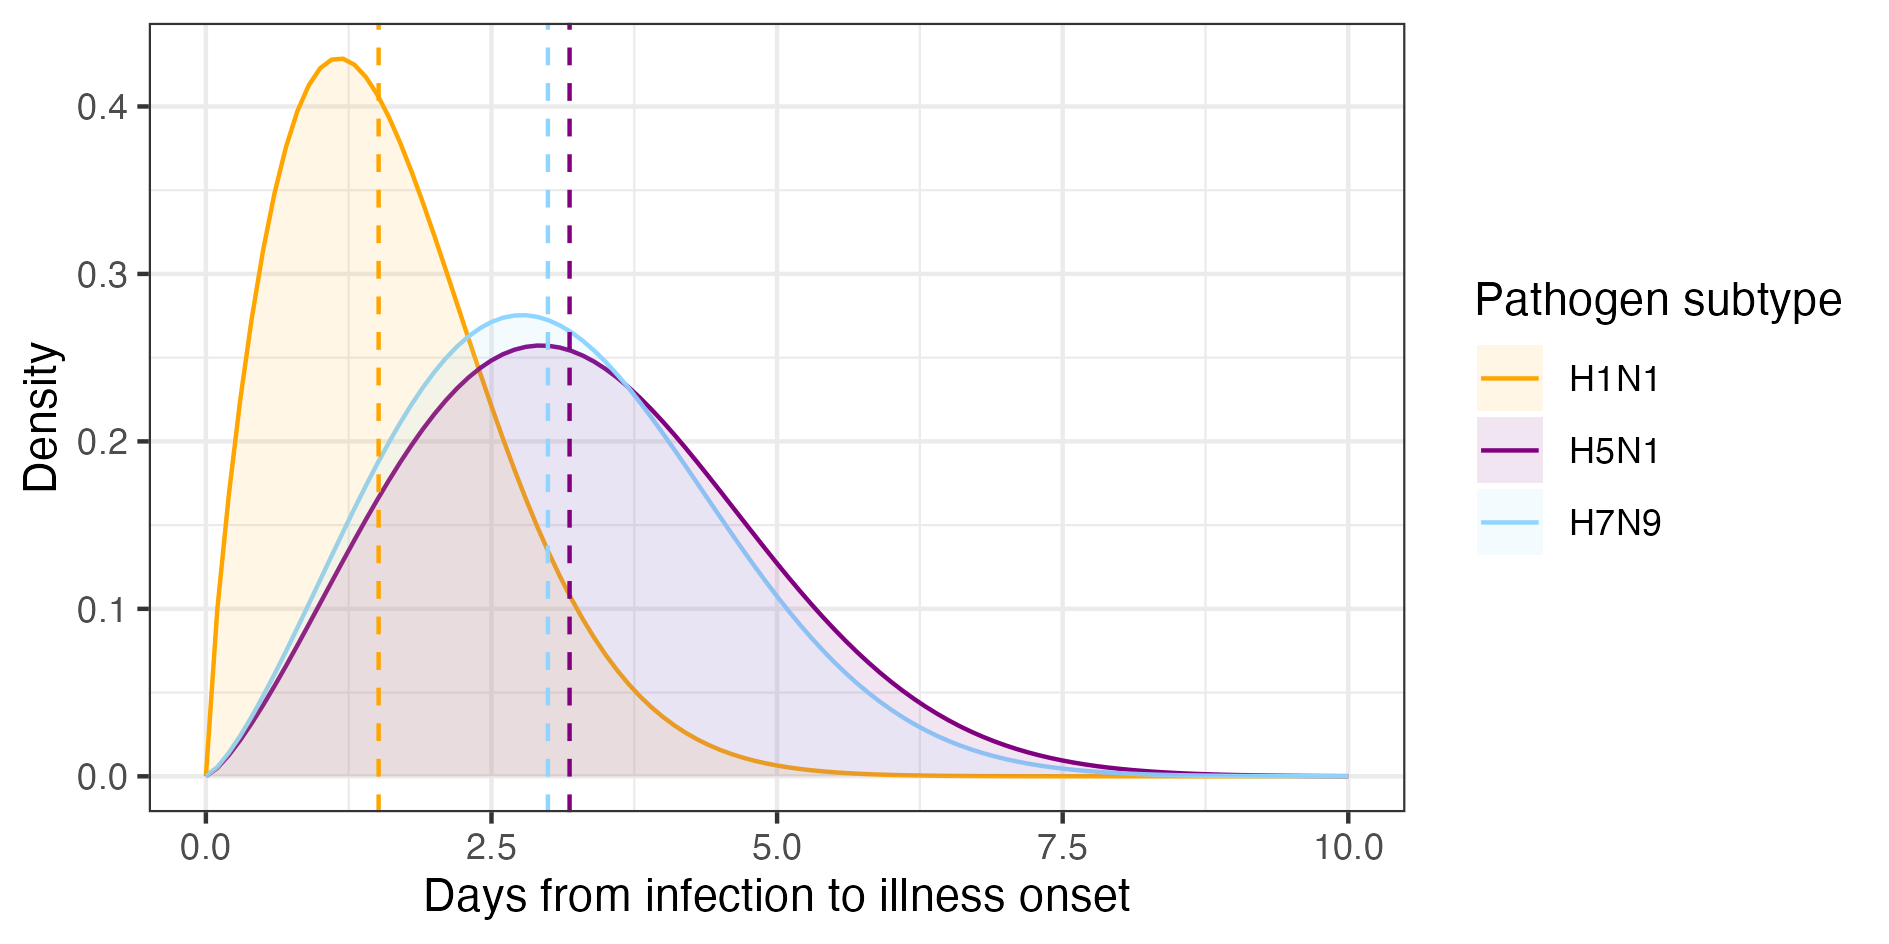
\includegraphics[width=\textwidth]{../plots/incubation_period.png}
\caption{Incubation period for the Influenza subtypes: H1N1, H5N1 and H7N9.}
\label{fig:incub}
\end{figure}

\begin{figure}[ht]
\centering
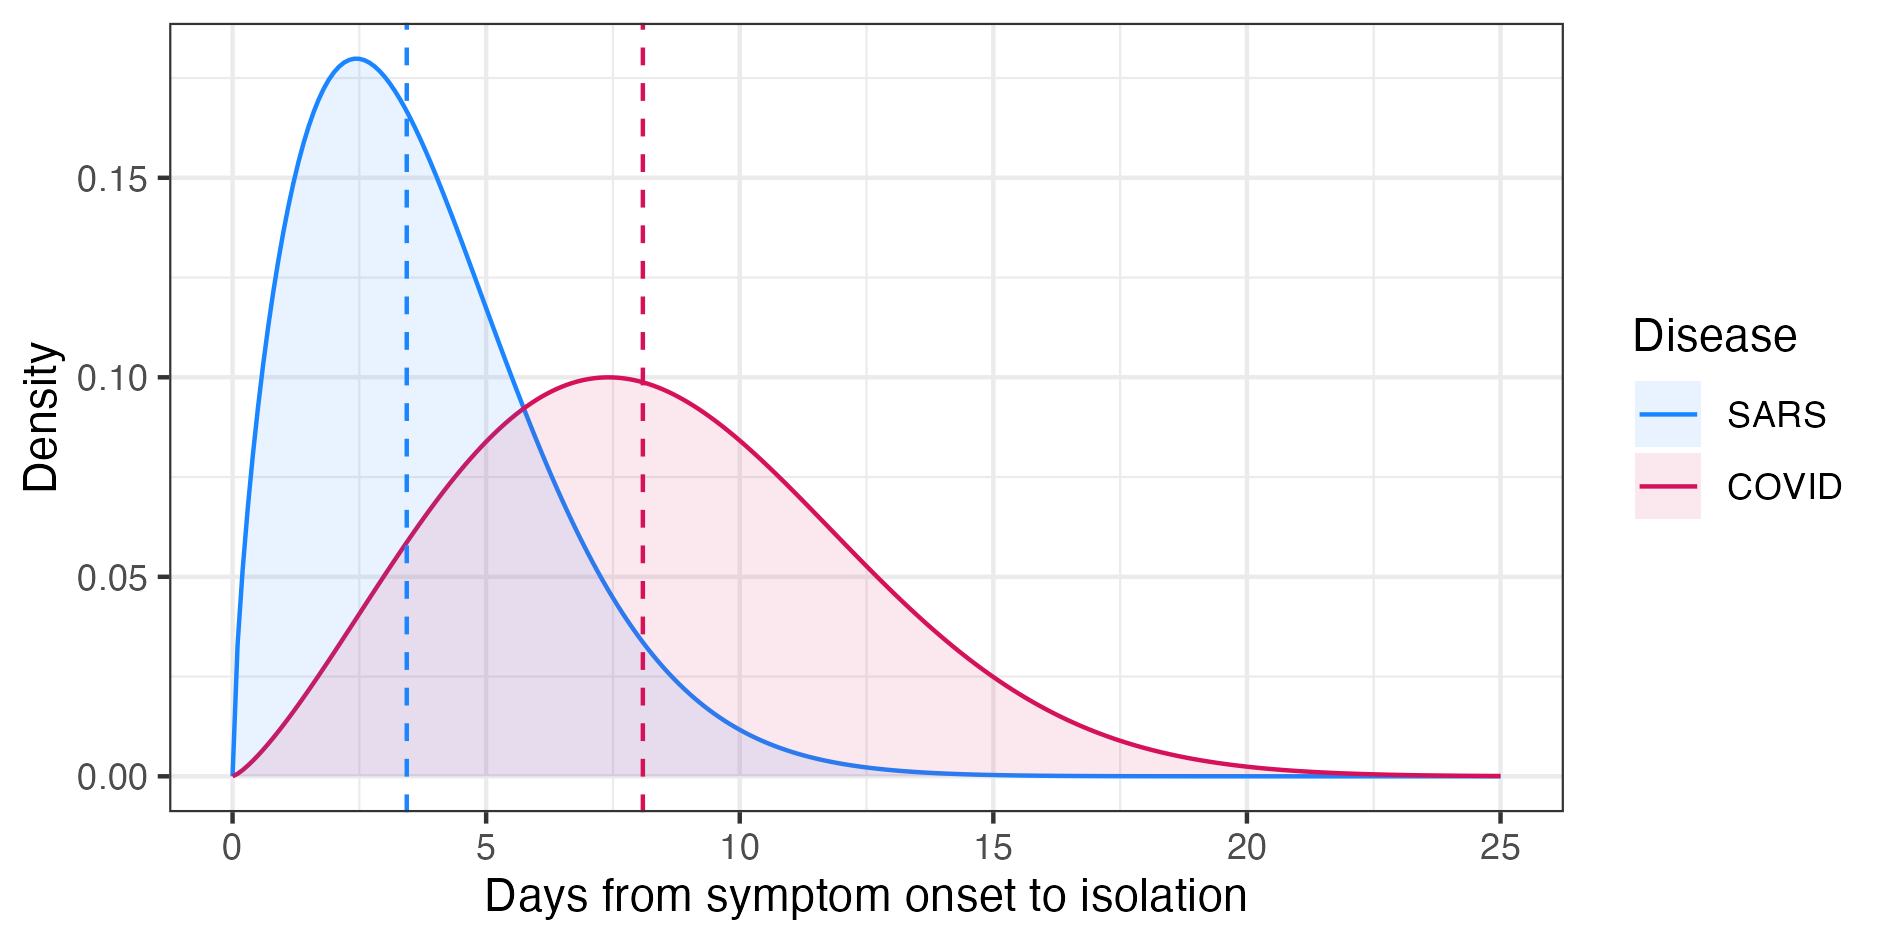
\includegraphics[width=\textwidth]{../plots/onset_to_isolation.png}
\caption{Onset-to-isolation delay distribution for SARS (SARS-CoV-1) and
  COVID-19 (SARS-CoV-2).}
\label{fig:onset-to-isolation}
\end{figure}


\begin{figure}[ht]
\centering
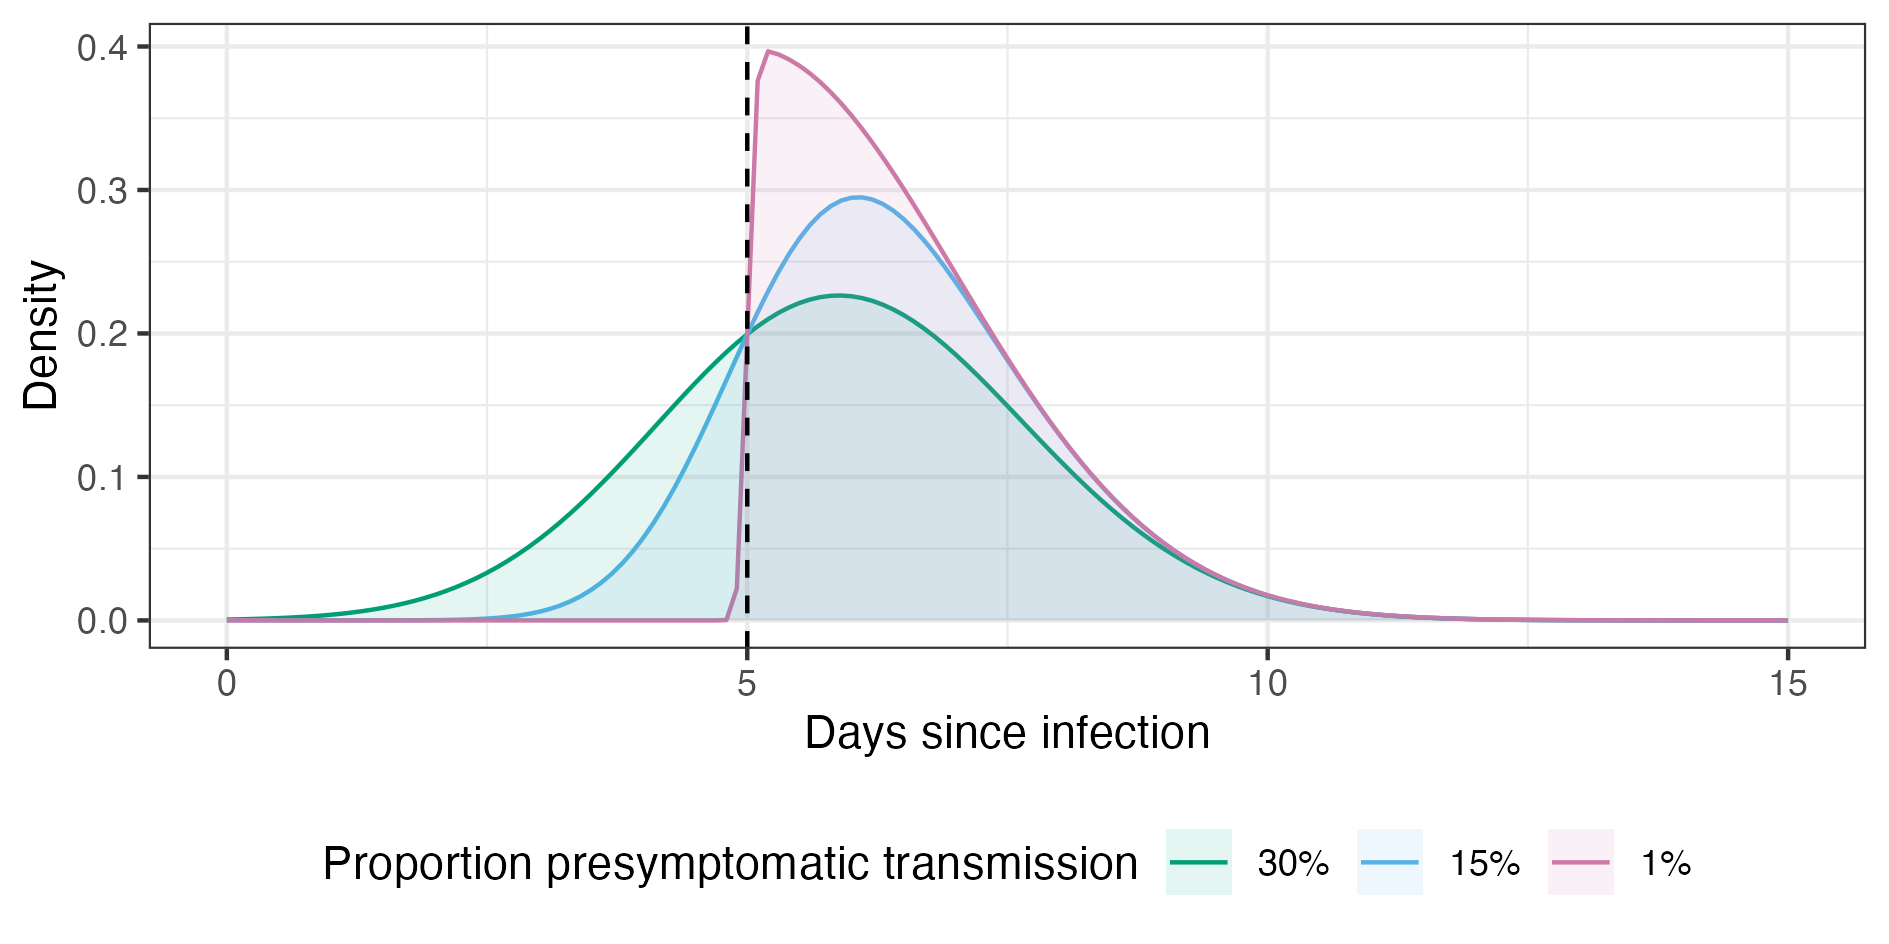
\includegraphics[width=\textwidth]{../plots/prop_presymptomatic_transmission.png}
\caption{Proportion of presymptomatic transmission determined by the incubation period, here assumed to be 5 days (dashed vertical line), controlled by a skewed-normal distribution.}
\label{fig:prop-presym-trans}
\end{figure}

We extract the incubation period or serial interval for each influenza subtype. We define the proportion of pre-symptomatic transmission as ... We define the onset-to-isolation delay distribution as short or long following the approach from \cite{hellewellFeasibilityControllingCOVID192020}.

\subsection*{Simulation scenarios}

We simulated scenarios with either 5 or 10 initial cases.

\section*{Results}

The incubation period for H1N1 is noticable shorter than the other two subtypes, which are similar, with H5N1 having a slightly longer median (Figure \ref{fig:incub}).

Predictably, a higher reproduction number for the outbreak results in a smaller percentage of outbreaks controlled at a given percentage of control effectiveness. (Figure \ref{fig:prop-outbreak-control-R}). The disparity of percentage outbreaks controlled becomes zero as the percentage of contacts traced exceeds 80\% (Figure \ref{fig:prop-outbreak-control-R}). When $R$ is only slightly above unity but below 2, the percentage of outbreaks controlled at 50\% of contacts traced and isolated is over 90\%, highlighting the effectiveness of this intervention for infectious diseases are not highly transmissible between humans.

\begin{figure}[ht]
\centering
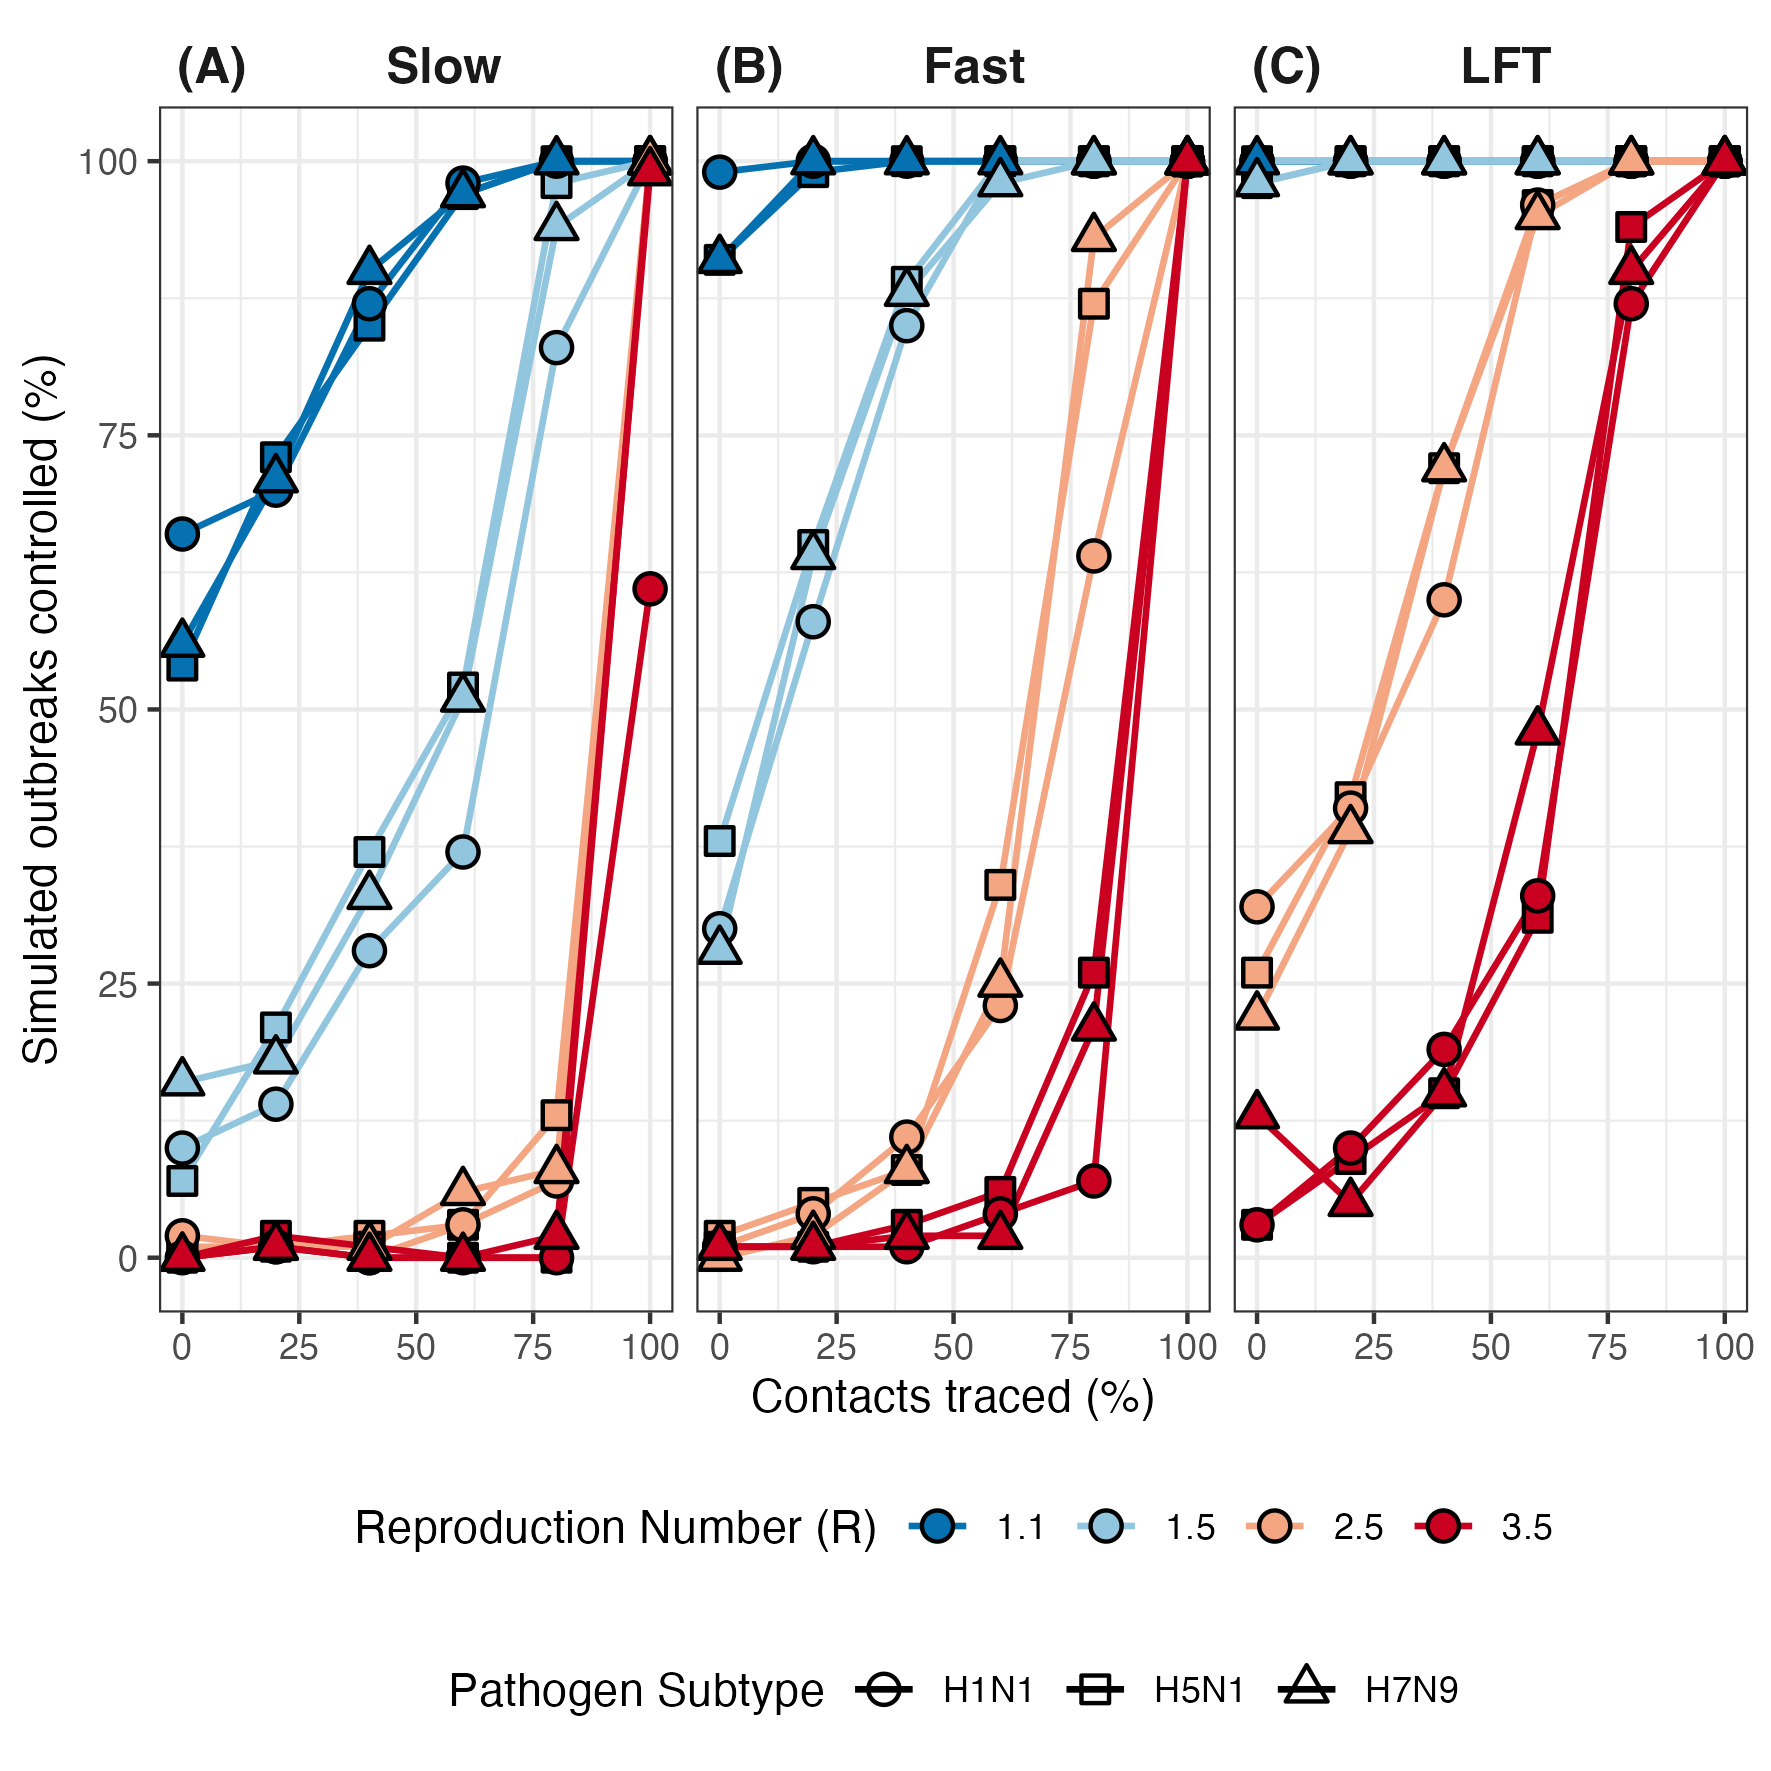
\includegraphics[width=\textwidth]{../plots/prop_outbreak_control_reproduction_number.png}
\caption{The percentage of outbreaks controlled across values of contact and isolation effectiveness, for outbreaks with an assumed reproduction number ($R$) of either 1.1 or 1.5. This is for a baselines scenario where the number of initial cases is 10, the proportion of presymptomatic transmission is 15\%, all cases are assumed symptomatic, and the onset-to-isolation delay is assumed to be SARS-like.}
\label{fig:prop-outbreak-control-R}
\end{figure}

\begin{figure}[ht]
\centering
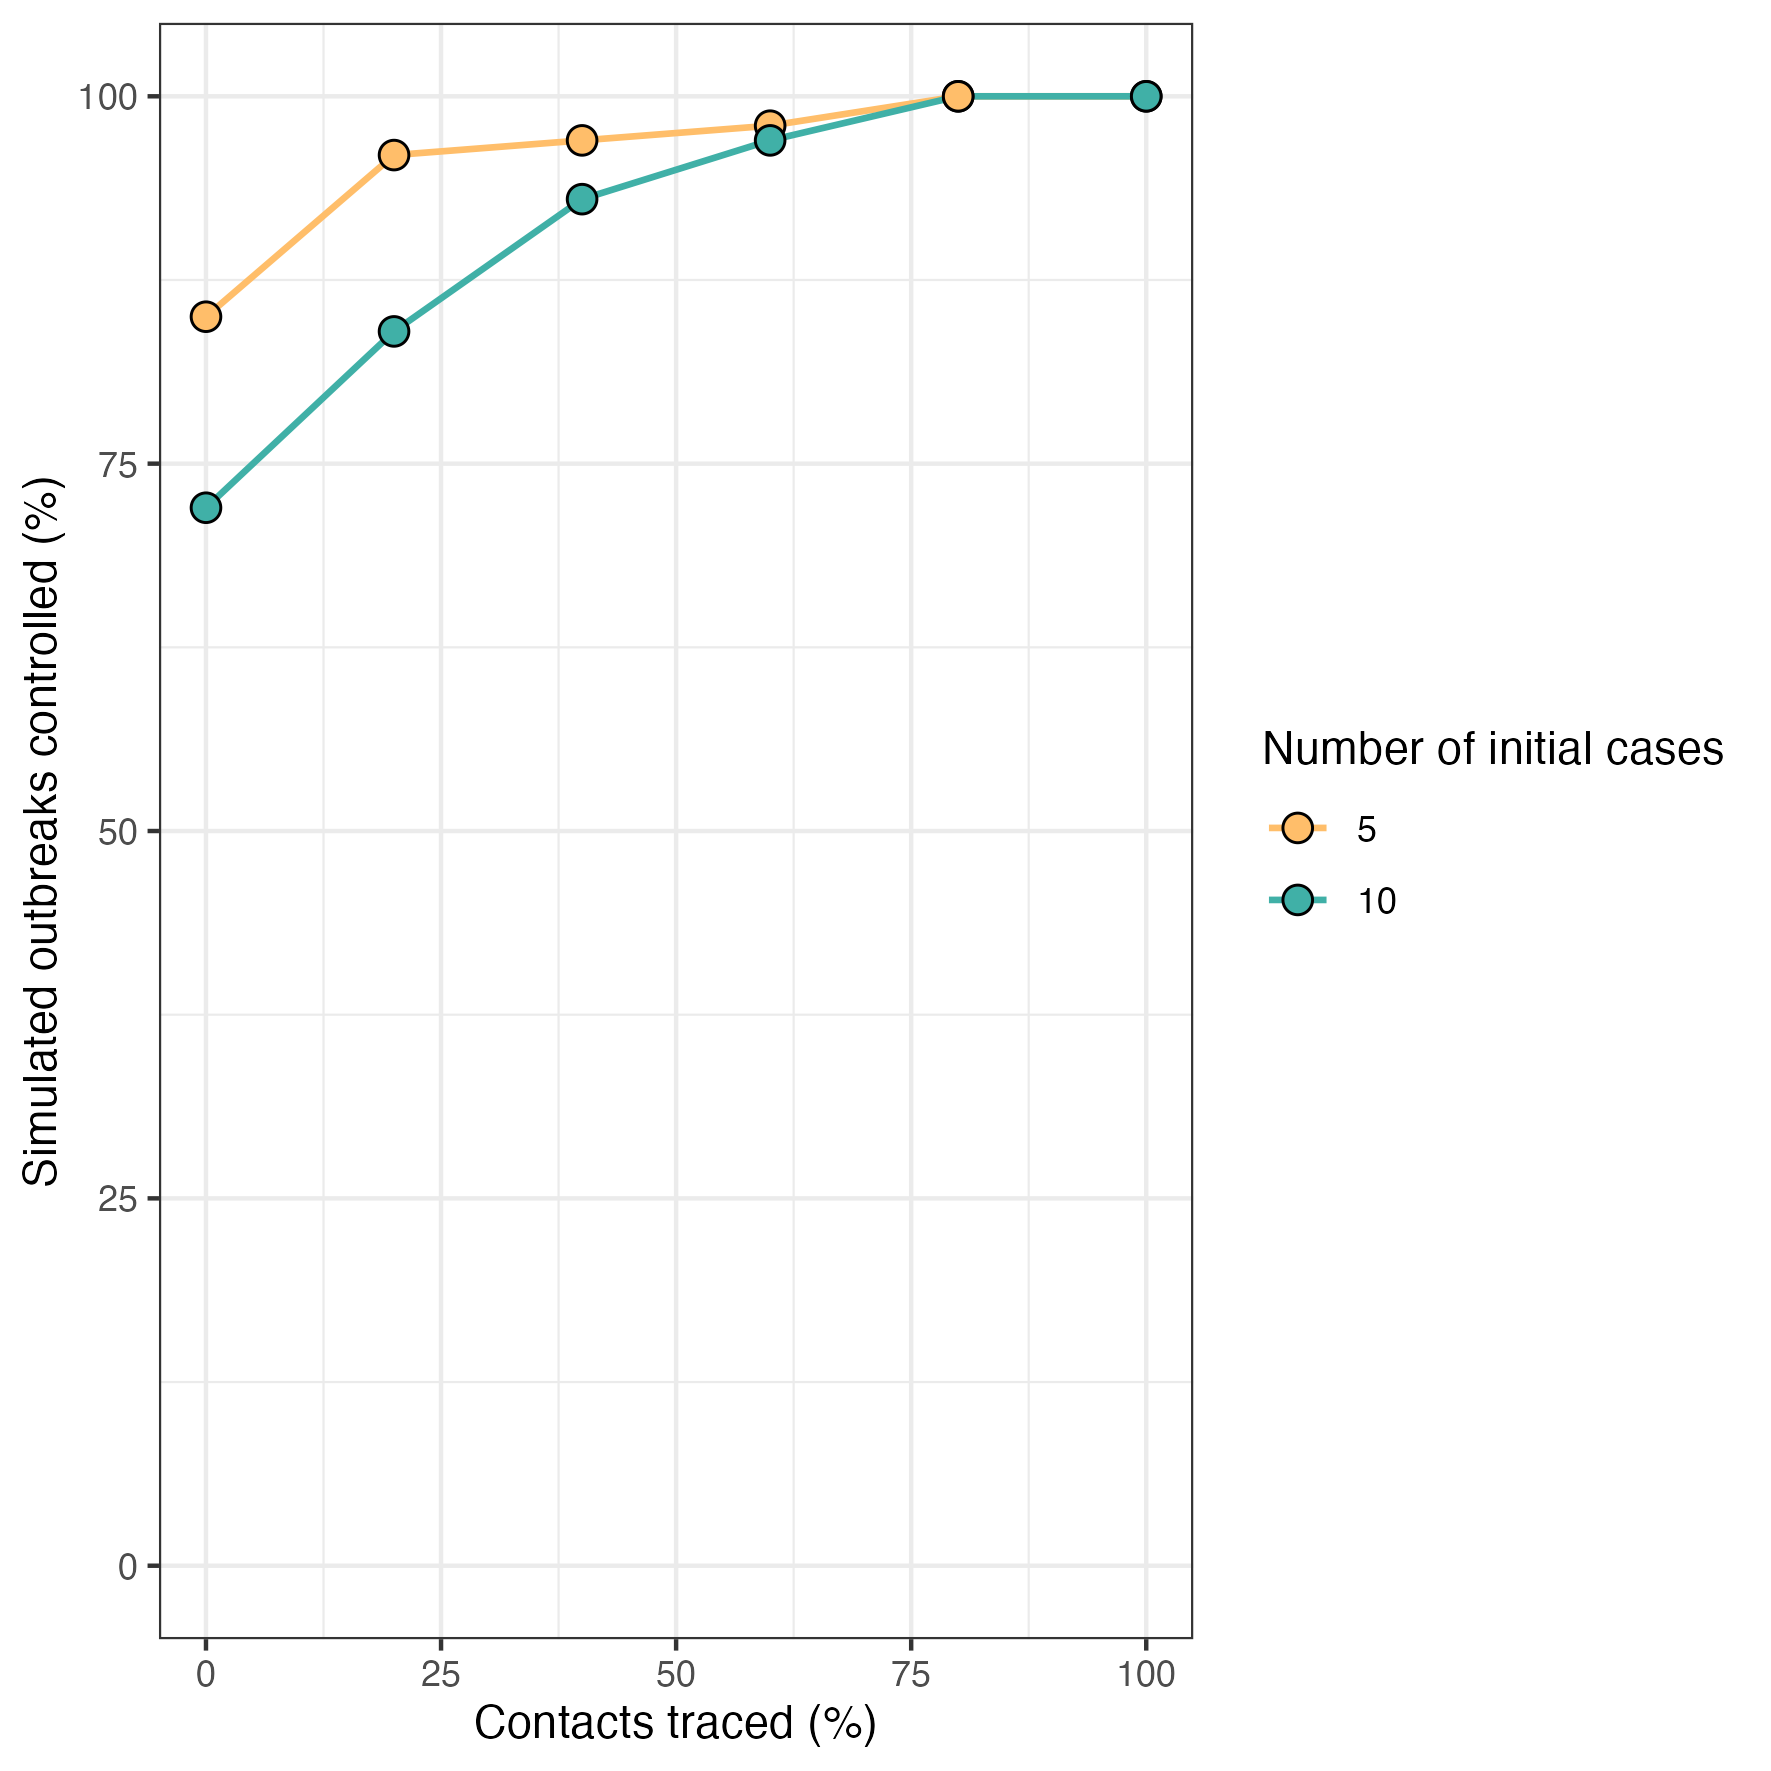
\includegraphics[width=\textwidth]{../plots/prop_outbreak_control_num_init_cases.png}
\caption{The percentage of outbreaks controlled across values of contact and isolation effectiveness, for outbreaks with an initial number of seeding infections assumed to be either 5 or 10. This is for a baselines scenario where the reproduction number is 1.5, the proportion of presymptomatic transmission is 15\%, all cases are assumed symptomatic, and the onset-to-isolation delay is assumed to be SARS-like.}
\label{fig:prop-outbreak-control-num-init-cases}
\end{figure}

\begin{figure}[ht]
\centering
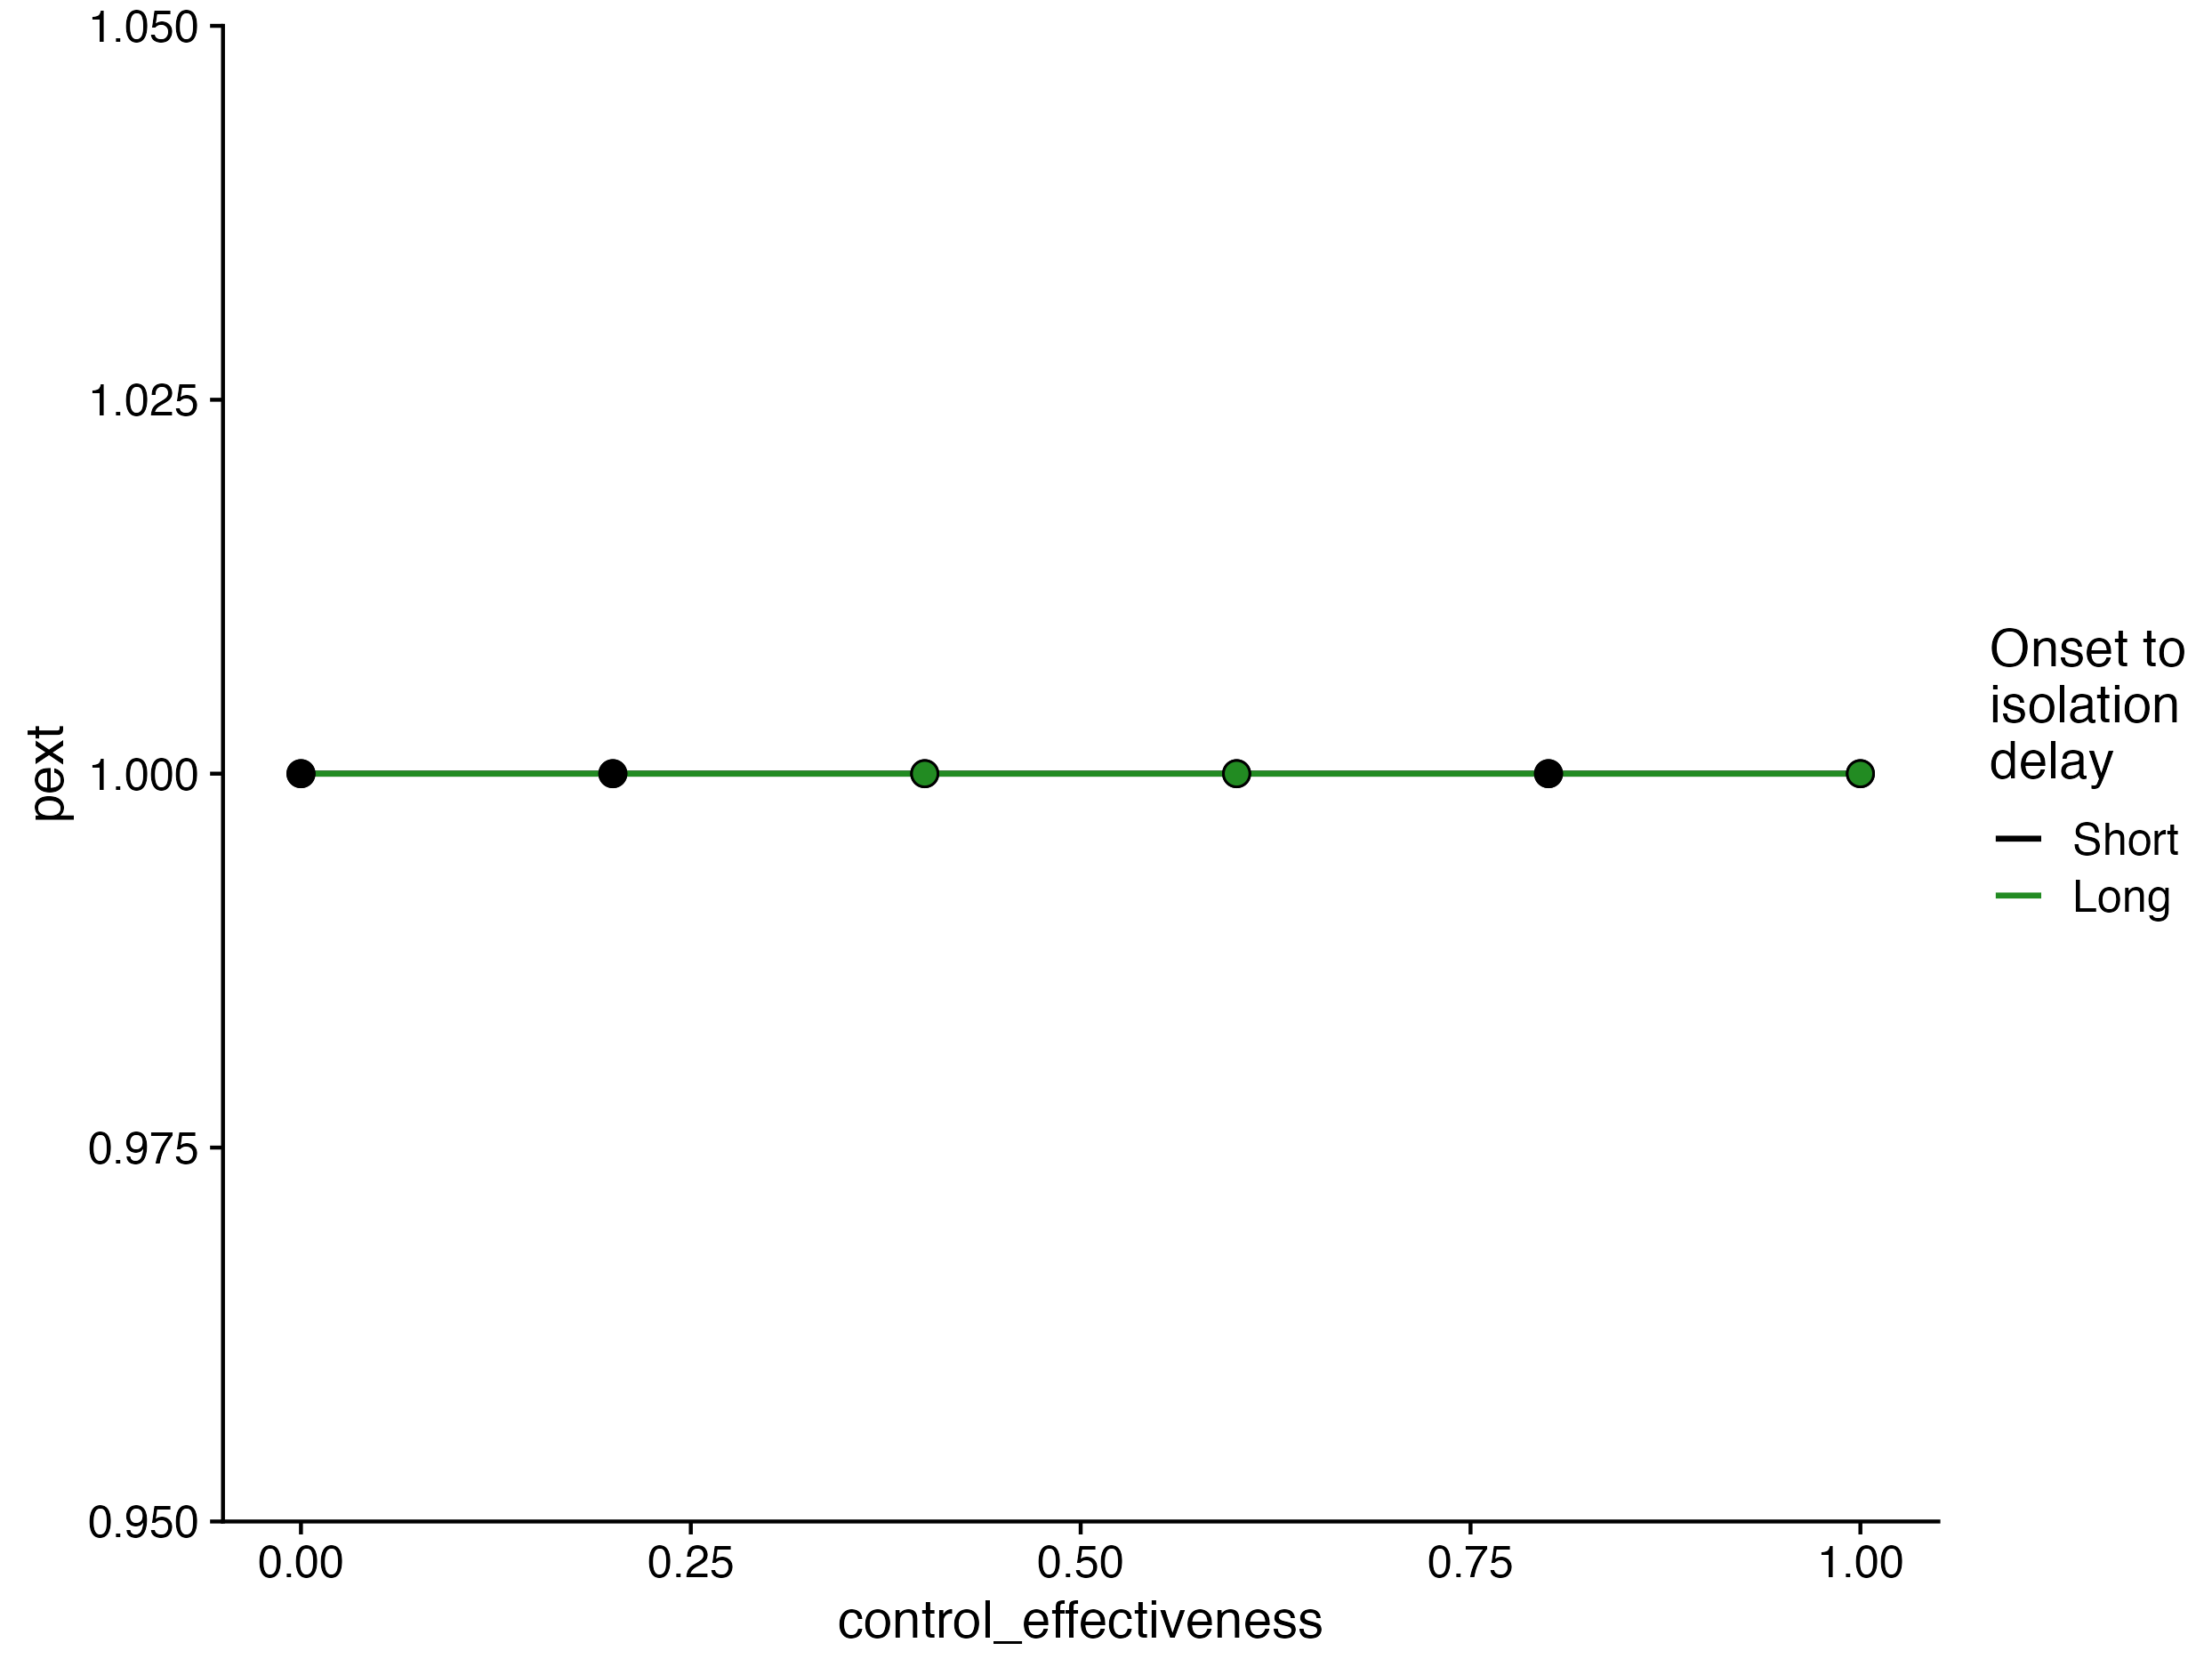
\includegraphics[width=\textwidth]{../plots/prop_outbreak_control_onset_to_isolation.png}
\caption{The percentage of outbreaks controlled across values of contact and isolation effectiveness, for outbreaks with an onset-to-isolation delay distribution that is either SARS-like, or COVID-19-like (from Wuhan). This is for a baselines scenario where the reproduction number is 1.5, the proportion of presymptomatic transmission is 15\%, all cases are assumed symptomatic, and the number of initial infections is 10.}
\label{fig:prop-outbreak-control-onset-to-isolation}
\end{figure}

\section*{Discussion}

\begin{itemize}
\item This study has looked at the feasibility and effectiveness of contact tracing and isolation for influenza subtypes that have cause epidemic outbreaks.
\item Discuss the existing flu vaccines and antivirals that can be used an interventions in addition to NPIs
\item In modelling the effectiveness of contact tracing and isolation we have assumed that there is no capacity limits on contact tracing, which does not hold in large outbreaks such as SARS-CoV-2 (ref). We also ignore potential socio-political factors that would prevent health worker from visiting or contacting infected individuals or contacts of infected individuals (Dhillon and Kelly, 2018). We also did not consider zoonotic spillover infections or formite transmission.
\item Digital tracing has capacity for large-scale contact tracing (pingdemic), also rapid tests are a complementary approach for limiting spread.
\item Antivirals for half the UK, these can be deployed in rapid response to flu pandemic.
\item In this study we have parameterised the transmission model with parameter from avian influenza subtypes (H5N1 and H7N9) and a influenza subtype that caused an epidemic in the recent past (H1N1), and response delays from SARS and COVID-19 outbreaks. However, these results can be used to inform other influenza subtypes that exhibit similar epidemiological characteristics in transmissibility and severity from past outbreaks (H2N2 and H3N2) and still exist in animal reservoirs for potential spillovers back into human populations (ref).
\end{itemize}

\bibliographystyle{plainnat}
\bibliography{FluTracer.bib}

\end{document}
